%%%%%%%%%%%%%%%%%%%%%%%%%%%%%%%%%%%%%%%%%%%%%%%%%%%
% CHƯƠNG 1: TỔNG QUAN VÀ CƠ SỞ LÝ THUYẾT
% = Gộp: Tổng quan UAV (cũ Ch1) + Cơ sở lý thuyết bay (cũ Ch2)
%%%%%%%%%%%%%%%%%%%%%%%%%%%%%%%%%%%%%%%%%%%%%%%%%%%
\section*{CHƯƠNG 1. TỔNG QUAN VÀ CƠ SỞ LÝ THUYẾT}
\addcontentsline{toc}{section}{\numberline{}CHƯƠNG 1. TỔNG QUAN VÀ CƠ SỞ LÝ THUYẾT}
\setcounter{section}{1}
\setcounter{subsection}{0}
\setcounter{figure}{0}
\setcounter{table}{0}

Chương này trình bày tổng quan về lĩnh vực UAV và các công nghệ liên quan, đồng thời xây dựng hệ thống cơ sở lý thuyết nền tảng làm căn cứ cho toàn bộ thiết kế phần cứng và phần mềm trong các chương tiếp theo. Nội dung bao gồm: khảo sát nghiên cứu trong và ngoài nước, phân tích các công nghệ được lựa chọn (STM32, ELRS, YOLOv8), mô hình động lực học Quadcopter, thuật toán bộ lọc bù tư thế, lý thuyết bộ điều khiển PID phân tầng và giao thức truyền thông không dây.

%%%% Phần 1.1--1.x: Tổng quan hệ thống Drone cứu hộ %%%%
% === NỘI DUNG: TỔNG QUAN HỆ THỐNG DRONE CỨU HỘ ===

\subsection{Tổng quan về UAV và ứng dụng trong cứu hộ cứu nạn}

Thiết bị bay không người lái (UAV -- Unmanned Aerial Vehicle) là một loại phương tiện hàng không được điều khiển từ xa hoặc hoạt động theo chương trình lập sẵn, không có phi công trên khoang. Trong những thập kỷ gần đây, UAV dân sự đã trải qua sự phát triển bùng nổ, từ các mô hình đơn giản dùng cho chụp ảnh trên không đến các hệ thống phức tạp tích hợp cảm biến đa phương thức và trí tuệ nhân tạo.

Theo phân loại hình thức cấu trúc khung thân, UAV dân sự phổ biến nhất hiện nay bao gồm:
\begin{itemize}
    \item \textbf{Quadcopter (4 cánh quạt)}: Cấu trúc đơn giản, dễ điều khiển, chi phí thấp, phù hợp cho các nhiệm vụ giám sát và cứu hộ tầm gần. Tiêu biểu là DJI Phantom, DJI Mavic và Parrot Anafi.
    \item \textbf{Hexacopter/Octocopter}: Cung cấp khả năng dự phòng động cơ và tải trọng lớn hơn, thường được dùng cho nhiệm vụ chuyên nghiệp như chụp ảnh điện ảnh hoặc giao hàng.
    \item \textbf{Fixed-wing UAV}: Hiệu quả năng lượng cao, tầm hoạt động xa, nhưng đòi hỏi không gian cất hạ cánh và không thể bay tại chỗ (hover).
    \item \textbf{Hybrid VTOL}: Kết hợp ưu điểm của cả hai loại trên, có khả năng cất hạ cánh thẳng đứng và chuyển đổi sang chế độ cánh cố định.
\end{itemize}

Trong lĩnh vực tìm kiếm cứu nạn (SAR -- Search and Rescue), Quadcopter được ưu tiên sử dụng nhờ khả năng hover ổn định tại chỗ, cơ động cao trong không gian hẹp, triển khai nhanh và chi phí đầu tư thấp. Các nghiên cứu gần đây \cite{Goodrich2008} chỉ ra rằng UAV có thể giảm thời gian tìm kiếm nạn nhân trong các vùng địa hình phức tạp xuống còn 15--20\% so với phương pháp truyền thống.

\begin{figure}[H]
    \centering
    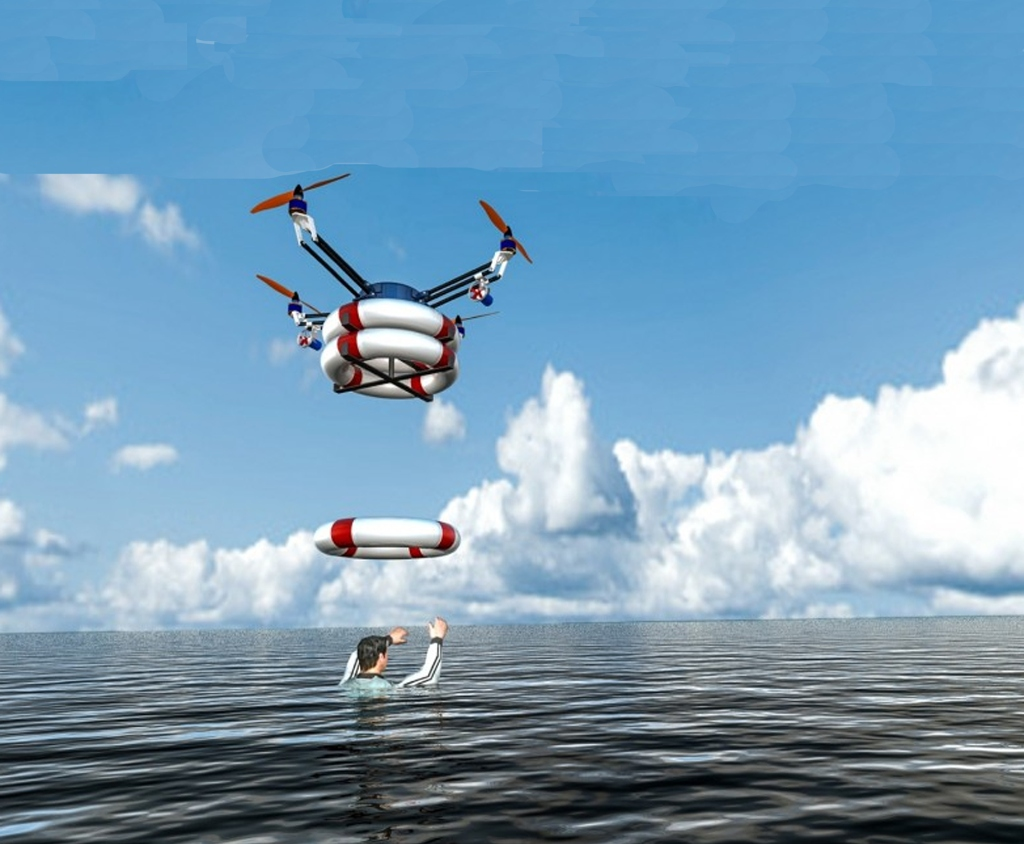
\includegraphics[width=0.8\textwidth]{Images/cuu_ho_sar.jpg}
    \caption[Hình ảnh minh họa hoạt động tìm kiếm cứu nạn bằng Drone]{\bfseries\fontsize{12pt}{0pt}\selectfont Hình ảnh minh họa hoạt động tìm kiếm cứu nạn bằng Drone}
    \label{fig:cuu_ho_sar}
\end{figure}


\subsection{Tình hình nghiên cứu trong và ngoài nước}

\subsubsection{Nghiên cứu quốc tế}

Trên thế giới, các nghiên cứu về UAV cứu hộ thông minh đã đạt được những kết quả đáng kể:

\begin{itemize}
    \item Hệ thống SHERPA (2013--2017) do Liên minh Châu Âu tài trợ đã phát triển đội UAV và UGV (robot mặt đất) phối hợp tìm kiếm nạn nhân trong các vụ lở tuyết, tích hợp camera nhiệt và nhận diện hình người \cite{DellAmore2014}.
    \item DJI và Parrot đã thương mại hóa các giải pháp UAV tích hợp camera nhiệt FLIR cho nhiệm vụ SAR ban đêm, được sử dụng rộng rãi bởi các đội cứu hộ tại Mỹ, Anh và Đức.
    \item Nghiên cứu của Bejiga et al. (2017) tại Na Uy đề xuất sử dụng mạng nơ-ron tích chập CNN để phát hiện người trong ảnh hồng ngoại từ UAV, đạt độ chính xác trên 85\% trong điều kiện tuyết trắng.
    \item Các nền tảng tự động bay phổ biến như ArduPilot (APM/Pixhawk) và Betaflight (cho FPV racing) đã cung cấp firmware mã nguồn mở cho cộng đồng nghiên cứu. Đề tài này lựa chọn phát triển firmware riêng trên STM32 để nắm sâu nguyên lý điều khiển.
\end{itemize}

\subsubsection{Nghiên cứu trong nước}

Tại Việt Nam, nghiên cứu về UAV cứu hộ đang trong giai đoạn phát triển:

\begin{itemize}
    \item Một số trường đại học như Đại học Bách Khoa Hà Nội, Học viện Kỹ thuật Quân sự đã nghiên cứu phát triển hệ thống điều khiển UAV dựa trên các nền tảng mã nguồn mở như ArduPilot và PX4.
    \item Tuy nhiên, phần lớn các nghiên cứu trong nước chủ yếu tập trung vào việc ứng dụng phần cứng thương mại sẵn có (Pixhawk, Naza-M) mà chưa đi sâu vào việc tự thiết kế Flight Controller từ đầu trên nền tảng vi điều khiển ARM nhúng.
    \item Hướng tích hợp AI -- cụ thể là YOLOv8 -- trực tiếp vào quy trình giám sát cứu hộ từ UAV vẫn là hướng nghiên cứu mới tại các trường kỹ thuật trong nước.
\end{itemize}

\subsection{Các công nghệ nền tảng được sử dụng trong đề tài}

\subsubsection{Vi điều khiển STM32F103C8T6 (ARM Cortex-M3)}

STM32F103C8T6 là vi điều khiển 32-bit thuộc dòng STM32F1 của STMicroelectronics, xây dựng trên lõi ARM Cortex-M3. Với tần số hoạt động tối đa 72\,MHz, bộ nhớ Flash 64\,KB, SRAM 20\,KB, đây là lựa chọn phổ biến cho các ứng dụng điều khiển nhúng thời gian thực nhờ khả năng xử lý mạnh mẽ, tiết kiệm năng lượng và hỗ trợ nhiều giao tiếp ngoại vi phong phú.

\begin{figure}[H]
    \centering
    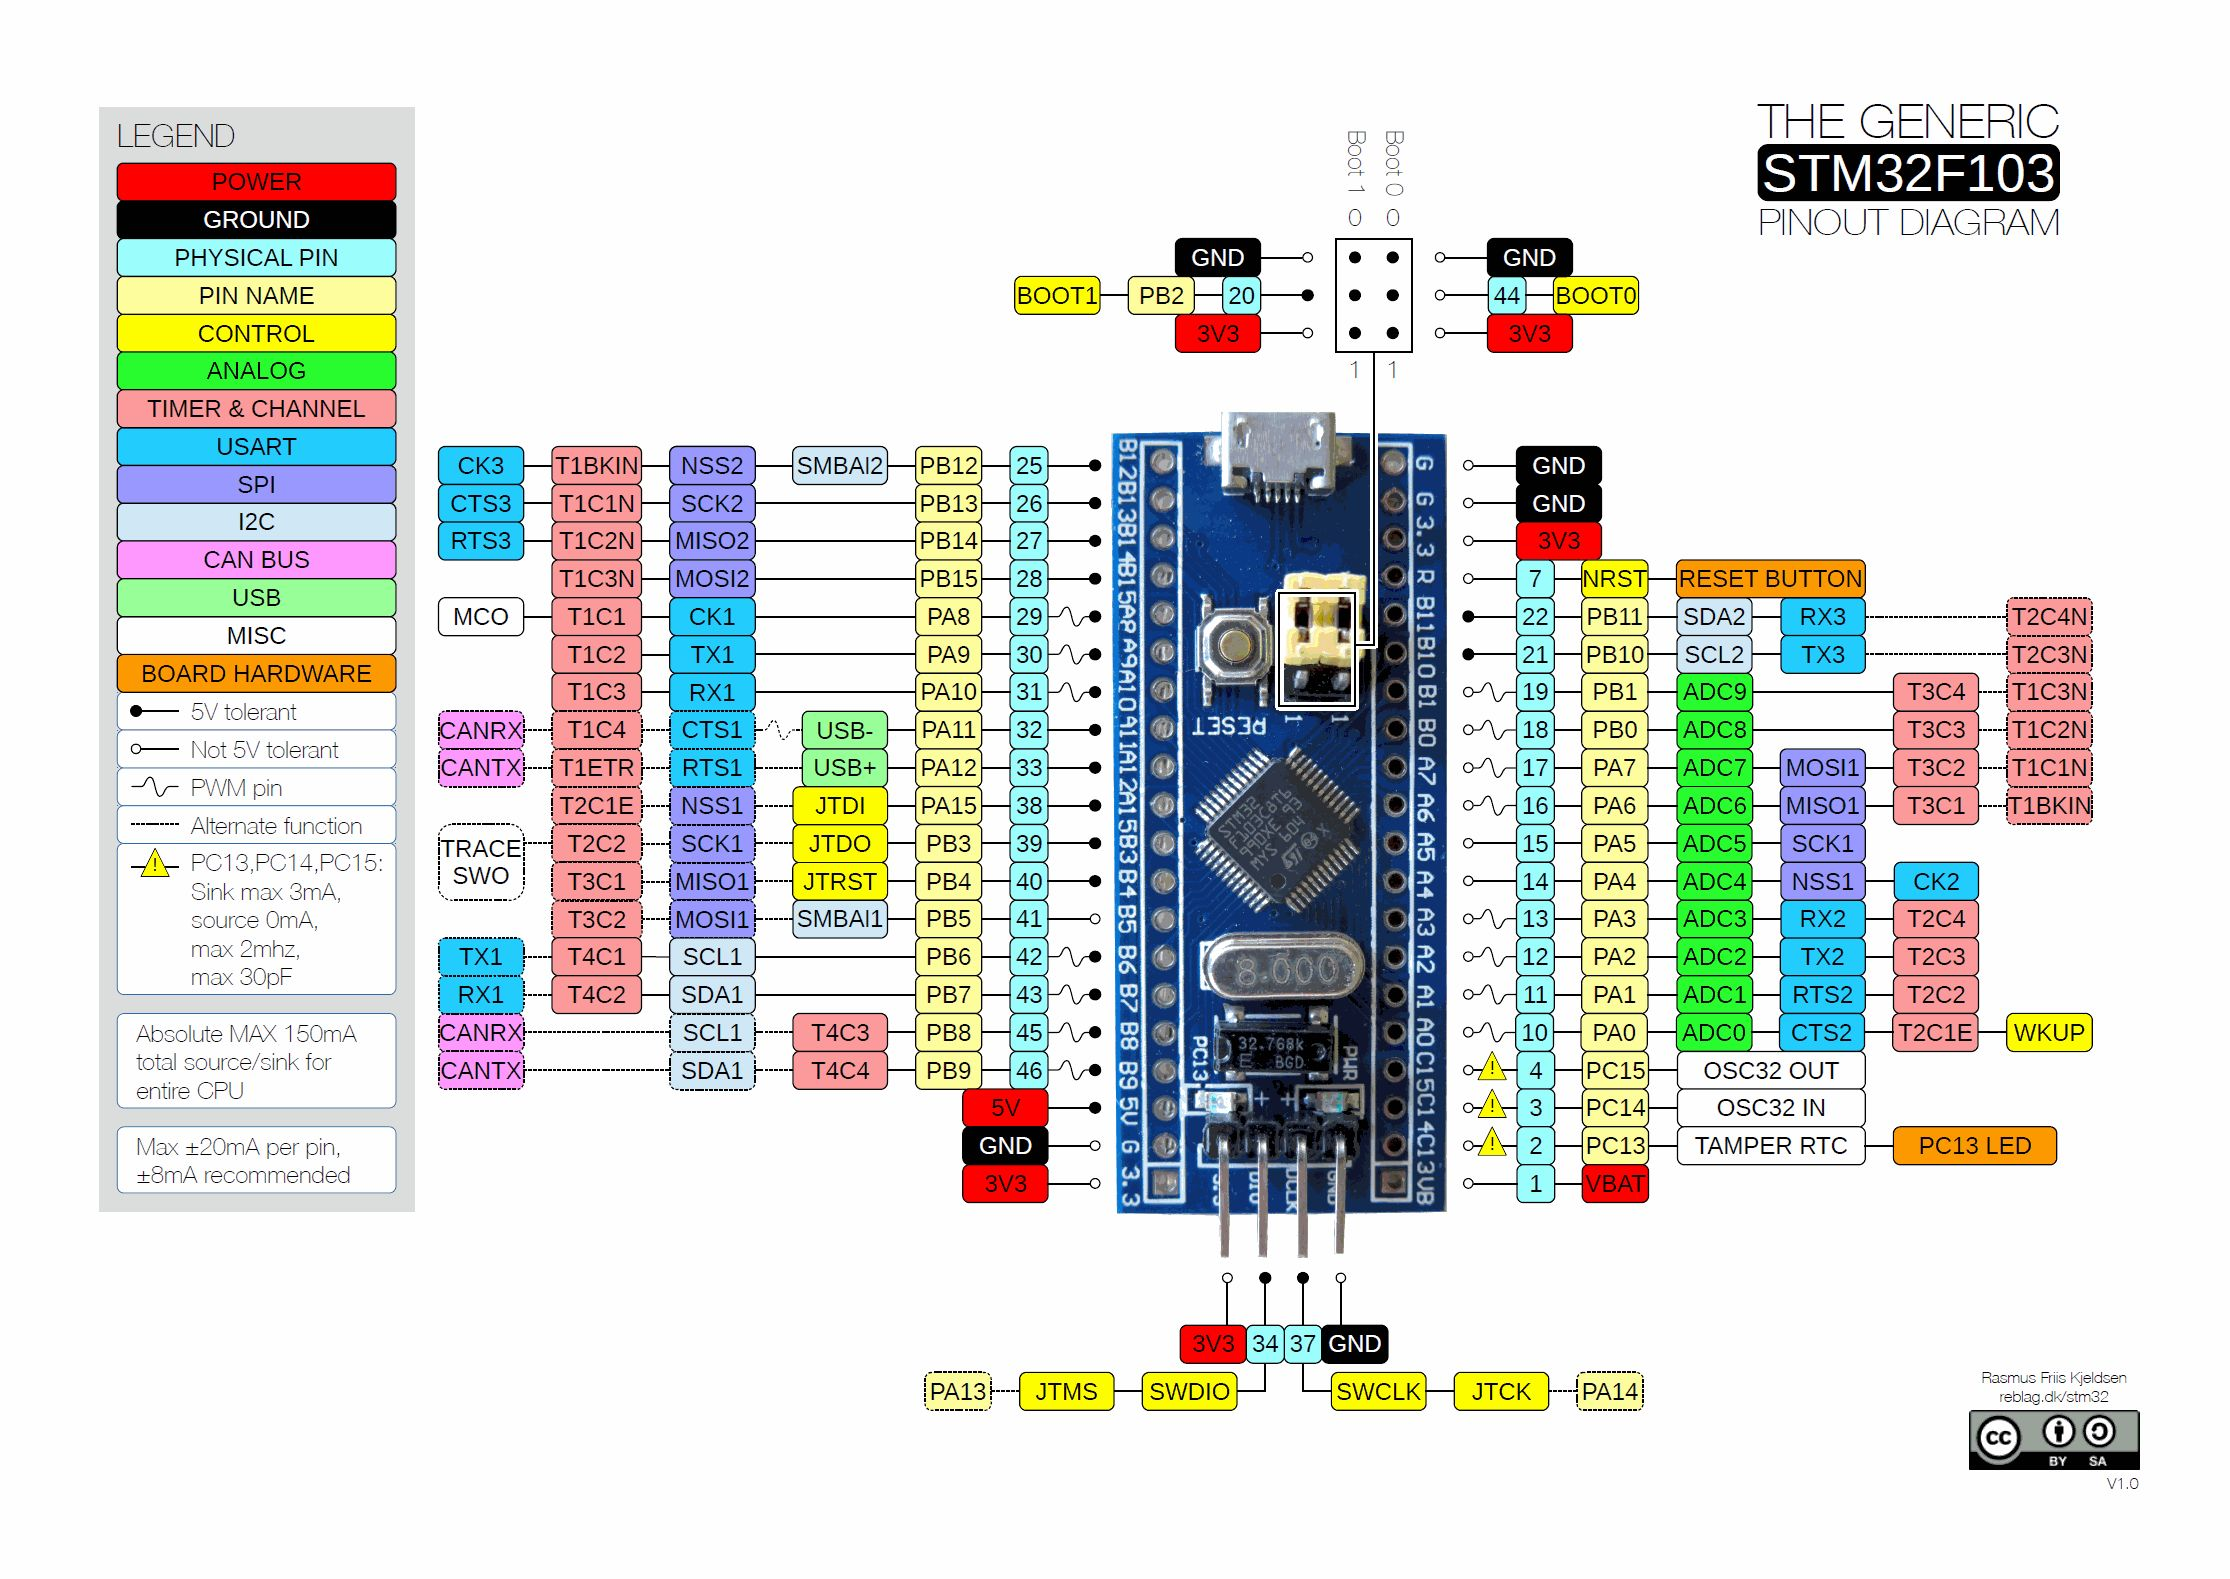
\includegraphics[width=0.6\textwidth]{Images/linhkien/stm32f103c8t6.jpg}
    \caption{Vi điều khiển STM32F103C8T6 (Dòng Blue Pill 48 chân)}
    \label{fig:stm32_ch1}
\end{figure}

\begin{table}[H]
    \centering
    \caption{Thông số kỹ thuật chính của STM32F103C8T6}
    \label{tab:stm32_specs}
    \begin{tabular}{|c|c|}
        \hline
        \textbf{Thông số} & \textbf{Giá trị} \\ \hline
        Bộ xử lý & ARM\textregistered\ Cortex\textregistered-M3 32-bit \\ \hline
        Tần số hoạt động & Lên đến 72\,MHz \\ \hline
        SRAM & 20\,KB \\ \hline
        Flash & 64\,KB \\ \hline
        Điện áp hoạt động & 2.0\,V -- 3.6\,V \\ \hline
        ADC & 2 bộ 12-bit (10 kênh đầu vào) \\ \hline
        UART & 3 bộ \\ \hline
        SPI & 2 bộ \\ \hline
        I2C & 2 bộ \\ \hline
        Số chân GPIO & Tối đa 37 chân (loại 48 chân) \\ \hline
    \end{tabular}
\end{table}

Trong đồ án này, STM32F103C8T6 được sử dụng làm bộ vi điều khiển trung tâm (Flight Controller) của toàn bộ hệ thống Drone. Mạch nhận nhiệm vụ thu thập dữ liệu góc thô từ cảm biến quán tính MPU6050 qua chuẩn giao tiếp I2C tốc độ cao, đồng thời đọc tín hiệu điều khiển từ bộ thu phát vô tuyến ELRS qua giao tiếp UART. Qua quá trình xử lý tín hiệu và tính toán thuật toán PID vòng lặp kép, chip vi điều khiển sẽ xuất xung PWM để điều khiển các động cơ không chổi than (thông qua ESC), giúp Drone giữ thăng bằng và phản hồi chính xác theo quỹ đạo điều khiển.

\subsubsection{Cảm biến quán tính IMU MPU6050}

MPU-6050 là module cảm biến quán tính 6-DoF (Degree of Freedom) của InvenSense, tích hợp đồng thời cảm biến gia tốc kế 3 trục (Accelerometer) và con quay hồi chuyển 3 trục (Gyroscope) trong cùng một chip. Giao tiếp qua giao thức I2C hoặc SPI. Chip này cũng tích hợp sẵn bộ xử lý tín hiệu số DMP (Digital Motion Processor) có thể ước lượng tư thế cơ bản, tuy nhiên trong đề tài ta sẽ đọc dữ liệu thô và tự cài đặt bộ lọc bù để nắm rõ nguyên lý.

\begin{figure}[H]
    \centering
    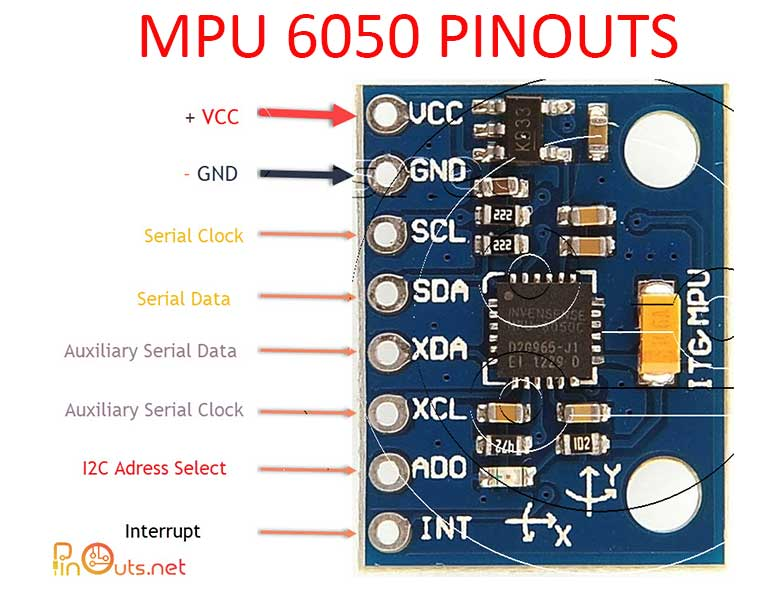
\includegraphics[width=0.45\textwidth]{Images/linhkien/mpu6050.jpg}
    \caption{Module cảm biến quán tính IMU MPU6050}
    \label{fig:mpu6050_ch1}
\end{figure}

\subsubsection{Giao thức điều khiển vô tuyến ExpressLRS (ELRS)}

Hệ thống điều khiển bay từ xa trong đồ án sử dụng giao thức truyền thông mã nguồn mở ExpressLRS (ELRS). Đây là giao thức thế hệ mới được thiết kế đặc biệt cho UAV FPV, nổi bật với:
\begin{itemize}
    \item Độ trễ cực thấp: 1--4\,ms tùy tốc độ packet.
    \item Tần số truyền gói điều khiển: lên đến 1000\,Hz ở chế độ 1000\,Hz Packet Rate.
    \item Phạm vi hoạt động lớn: tới vài km với công suất phát 250\,mW.
    \item Chuẩn giao tiếp với FC: giao thức CRSF (Crossfire Serial) trên UART.
\end{itemize}

Hệ thống điều khiển bao gồm hai thiết bị chính:

\paragraph{Tay điều khiển phát sóng (TX - RadioMaster Pocket)}

Tay cầm điều khiển (Transmitter) RadioMaster Pocket được tích hợp sẵn module phát sóng ELRS tần số 2.4\,GHz. Thiết bị này đọc vị trí góc nghiêng của các cần gạt (joystick), mã hóa thành gói tin CRSF và truyền đi với độ trễ cực thấp. Thiết bị hỗ trợ tốc độ truyền gói tin điều khiển cực cao (lên tới 500\,Hz) với công suất phát linh hoạt, mang lại độ nhạy sóng cao và cự ly điều khiển ổn định đạt hàng kilômét trong điều kiện khuất địa hình.
\begin{figure}[H]
    \centering
    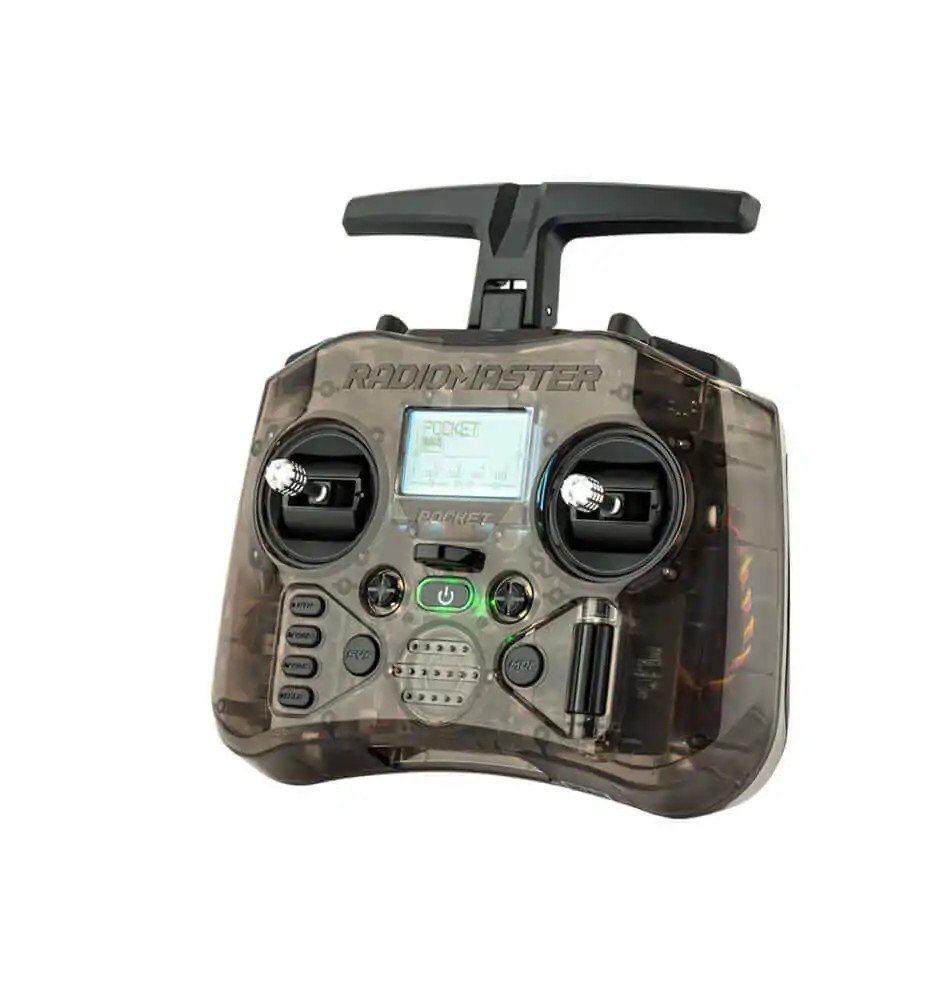
\includegraphics[width=0.45\textwidth]{Images/rm_pocket.png}
    \caption{Tay điều khiển phát sóng RadioMaster Pocket (TX)}
    \label{fig:rm_pocket_ch1}
\end{figure}

\paragraph{Module thu sóng (RX - Cyclone ELRS 2.4GHz 7CH)}

Mạch thu sóng siêu nhỏ (Receiver) được lắp đặt trực tiếp trên Drone. Module có nhiệm vụ nhận gói tin tần số cao từ tay phát và kết nối với Flight Controller thông qua giao thức truyền thông UART nối tiếp tốc độ cao sử dụng chuẩn giao thức CRSF (Crossfire) với tốc độ baud mặc định là 420.000\,bps. Dòng dữ liệu nối tiếp nguyên bản sẽ được đẩy vào vi điều khiển STM32F103C8T6 để giải mã lệnh bay, giúp giảm thiểu tối đa độ trễ.
\begin{figure}[H]
    \centering
    
\includegraphics[width=0.4\textwidth]{Images/linhkien/elrs_rx.png}
    \caption{Module thu tín hiệu vô tuyến ExpressLRS (RX)}
    \label{fig:elrs_rx_ch1}
\end{figure}

\subsubsection{Camera FPV và hệ thống truyền hình ảnh VTX/VRX}

Hệ thống truyền hình ảnh analog FPV (First-Person View) trong đồ án đóng vai trò thu thập và truyền tải video thời gian thực từ Drone về trạm mặt đất để phục vụ mô hình AI phân tích. Hệ thống bao gồm 3 thành phần chính:

\paragraph{Camera FPV (Caddx Ant Lite)}

Camera Caddx Ant Lite chuyên dụng cho thiết bị bay sở hữu cảm biến CMOS 1/3 inch, độ phân giải sắc nét 1200\,TVL và tích hợp dải động cao Global WDR giúp duy trì khả năng quan sát tốt nạn nhân trong môi trường ngược sáng mạnh. Trọng lượng camera siêu nhẹ (2\,g) và độ trễ truyền dẫn tín hiệu analog gần như bằng 0 (dưới 10\,ms) là các yếu tố then chốt cho hệ thống FPV. Camera xuất trực tiếp tín hiệu video analog chuẩn NTSC/PAL với độ nhạy sáng cao.
\begin{figure}[H]
    \centering
    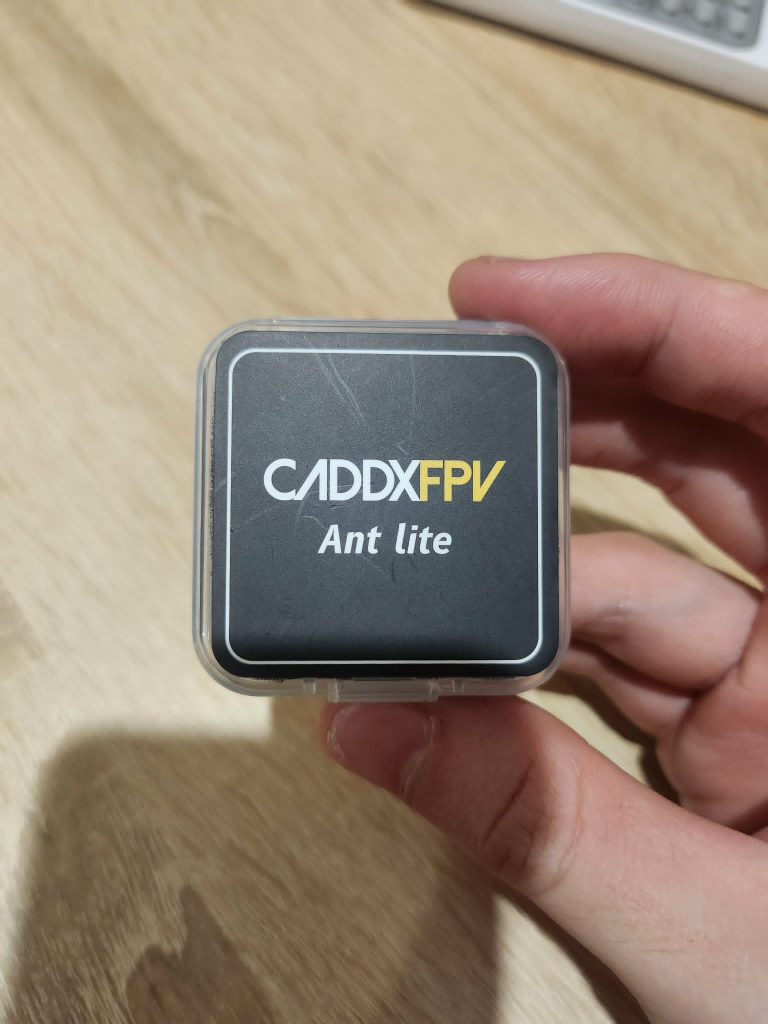
\includegraphics[width=0.35\textwidth]{Images/caddx_cam.png}
    \caption{Camera FPV Caddx Ant Lite}
    \label{fig:caddx_cam_ch1}
\end{figure}

\paragraph{Module phát video VTX (Cyclone VTX 5.8GHz)}

Cyclone VTX là module phát sóng video analog hoạt động ở băng tần 5.8\,GHz. Mạch có công suất phát tối đa lên tới 1000\,mW để truyền tín hiệu từ camera về trạm mặt đất. Thiết bị hỗ trợ phím nhấn vật lý kết hợp LED trạng thái trực quan để chuyển đổi linh hoạt giữa các dải tần số (Band A/B/E/F/R), các kênh phát (CH1-CH8) và mức công suất (25/100/200/400/1000\,mW), giúp người vận hành dễ dàng tối ưu hóa chất lượng sóng truyền hình ảnh và tránh hiện tượng nhiễu xuyên kênh.
\begin{figure}[H]
    \centering
    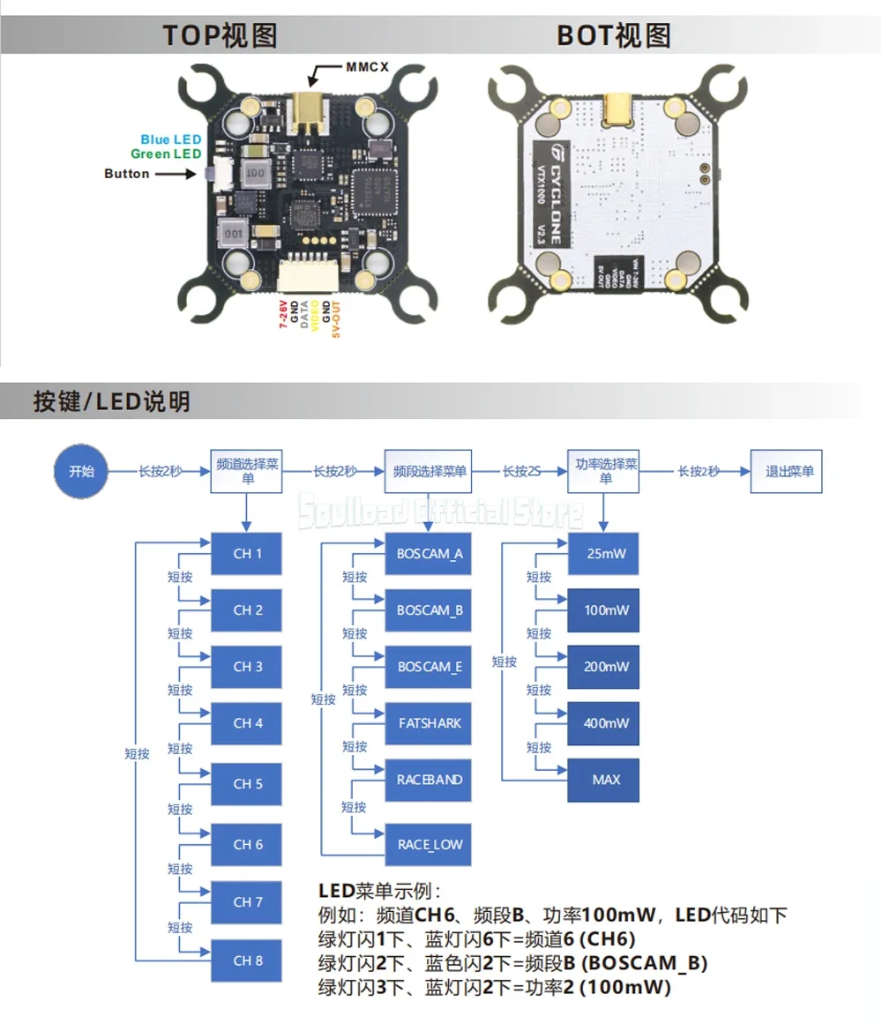
\includegraphics[width=0.4\textwidth]{Images/cyclone_vtx.png}
    \caption{Module phát hình ảnh Cyclone VTX 5.8GHz}
    \label{fig:cyclone_vtx_ch1}
\end{figure}

\paragraph{Module thu video VRX (Skydroid 5.8G OTG)}

Trạm mặt đất sử dụng bộ thu hình chuyên dụng Skydroid 5.8G OTG Receiver. Bộ thu tự động dò quét và đồng bộ hóa tần số phát sóng của VTX qua 150 kênh sóng. Video thu được được chuyển đổi sang chuẩn tín hiệu số và truyền trực tiếp vào máy tính trạm mặt đất GCS thông qua kết nối USB dạng UVC (OTG), giúp phần mềm AI Python dễ dàng đọc luồng video và thực thi nhận diện mà không cần thêm thiết bị Capture rời nào.
\begin{figure}[H]
    \centering
    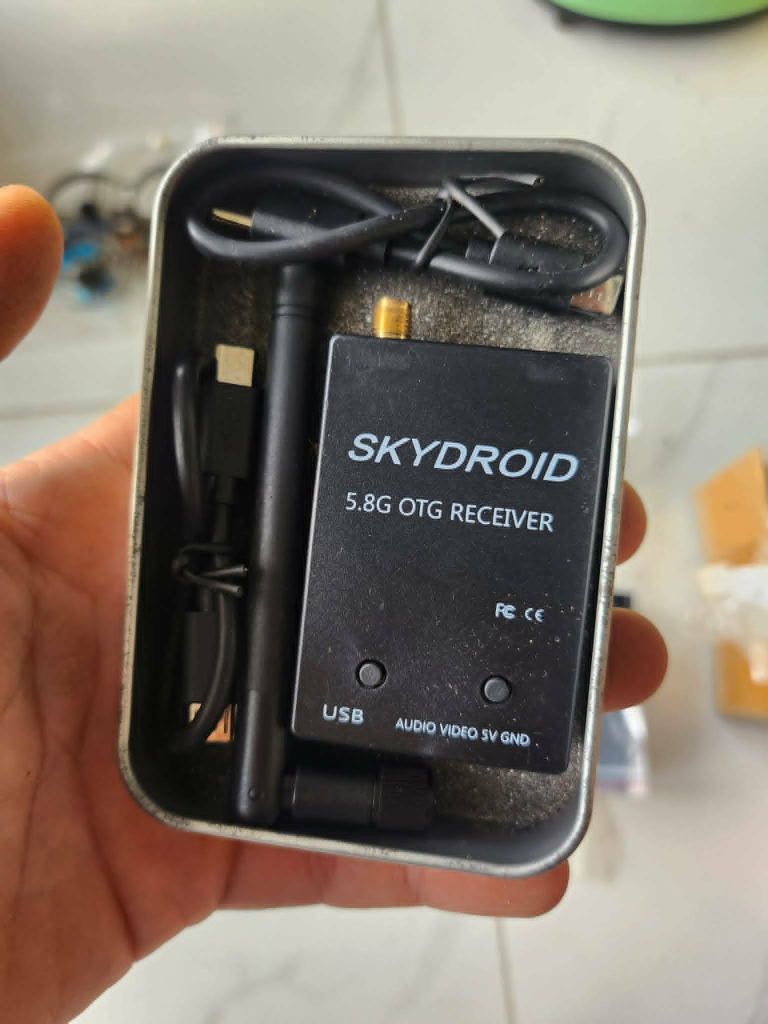
\includegraphics[width=0.4\textwidth]{Images/skydroid_vrx.png}
    \caption{Thiết bị thu và số hóa hình ảnh Skydroid 5.8G OTG VRX}
    \label{fig:skydroid_vrx_ch1}
\end{figure}

Việc sử dụng trọn bộ hệ thống analog FPV này mang lại ưu điểm vượt trội về độ trễ đầu cuối (end-to-end latency thấp hơn 40\,ms) so với các giải pháp IP Camera kỹ thuật số, hoàn toàn đáp ứng được yêu cầu cập nhật theo thời gian thực của thuật toán phát hiện nạn nhân.



\subsection{Xác định khoảng trống nghiên cứu và hướng tiếp cận của đề tài}

Qua phân tích tổng quan, có thể nhận thấy các khoảng trống nghiên cứu sau:

\subsubsection{Thiếu nghiên cứu tự thiết kế FC nhúng ARM cho UAV cứu hộ trong nước}
Phần lớn đề tài trong nước dùng FC thương mại, không đi sâu vào thiết kế phần cứng từ đầu. Đề tài này lấp đầy khoảng trống này bằng cách tự thiết kế PCB và lập trình firmware hoàn toàn trên STM32F103.

\subsubsection{Thiếu hệ thống AI đa mô hình dung hợp quyết định cho bài toán cứu hộ}
Các nghiên cứu hiện tại thường chỉ dùng một mô hình đơn lẻ (phát hiện người) mà chưa kết hợp đa mô hình đánh giá trạng thái nguy hiểm. Đề tài đề xuất thuật toán dung hợp ba mô hình YOLOv8 tính Danger Score toàn cục.

\subsubsection{Thiếu tích hợp từ đầu đến cuối}
Phần cứng Drone và hệ thống AI thường được nghiên cứu tách biệt. Đề tài này cung cấp một giải pháp tích hợp từ thiết kế cơ khí, điện tử đến phần mềm AI, tạo thành một hệ thống hoàn chỉnh.

\textbf{Hướng tiếp cận} của đề tài là kết hợp phương pháp từ dưới lên (Bottom-up): bắt đầu từ thiết kế linh kiện phần cứng cơ bản, xây dựng lớp firmware điều khiển thời gian thực, sau đó phát triển lớp AI ở cấp độ trạm mặt đất, và cuối cùng tích hợp thành hệ thống hoàn chỉnh để thử nghiệm trong điều kiện thực tế.


\bigskip
%%%% Phần 1.x+1--: Cơ sở lý thuyết điều khiển bay %%%%
%%%%%%%%%%%%%%%%%%%%%%%%%%%%%%%%%%%%%%%%%%%%%%%%%%%
% CHƯƠNG 2: CƠ SỞ LÝ THUYẾT VỀ HỆ THỐNG BAY VÀ ĐIỀU KHIỂN NHÚNG
%%%%%%%%%%%%%%%%%%%%%%%%%%%%%%%%%%%%%%%%%%%%%%%%%%%
\section*{CHƯƠNG 2. CƠ SỞ LÝ THUYẾT VỀ HỆ THỐNG BAY VÀ ĐIỀU KHIỂN NHÚNG}
\addcontentsline{toc}{section}{\numberline{}CHƯƠNG 2. CƠ SỞ LÝ THUYẾT VỀ HỆ THỐNG BAY VÀ ĐIỀU KHIỂN NHÚNG}
\setcounter{section}{2}
\setcounter{subsection}{0}
\setcounter{figure}{0}
\setcounter{table}{0}

\subsection{Động lực học Quadcopter và Hệ tọa độ bay}

Thiết bị Quadcopter là một hệ thống động lực phi tuyến phức tạp gồm 4 động cơ xoay chổi than/không chổi than đặt đối xứng tại các đỉnh của khung chữ X hoặc chữ thập. Chuyển động bay của Quadcopter được kiểm soát trực tiếp bằng cách thay đổi vận tốc quay của 4 cánh quạt độc lập.

Để mô tả trạng thái chuyển động của thiết bị bay, ta sử dụng hai hệ tọa độ tiêu chuẩn:
\begin{enumerate}
    \item \textbf{Hệ tọa độ Trái Đất (Inertial Frame - Earth Frame - $E$)}: Là hệ tọa độ cố định gắn với mặt đất, dùng làm mốc quy chiếu vị trí không gian của Drone.
    \item \textbf{Hệ tọa độ vật thể (Body Frame - $B$)}: Có tâm trùng với trọng tâm của Drone. Trục X hướng dọc về phía trước (Front/Roll), trục Y hướng sang bên phải (Right/Pitch), trục Z vuông góc với mặt phẳng bay hướng lên trên hoặc xuống dưới tùy cấu hình (Yaw).
\end{enumerate}

Sự định hướng của hệ tọa độ Body frame so với Earth frame được mô tả bằng ba góc Euler: góc Roll ($\phi$, nghiêng cánh quanh trục X), góc Pitch ($\theta$, chúi mũi quanh trục Y), và góc Yaw ($\psi$, xoay mũi quanh trục Z) như minh họa trong Hình \ref{fig:he_toa_do_drone}.

\begin{figure}[H]
    \centering
    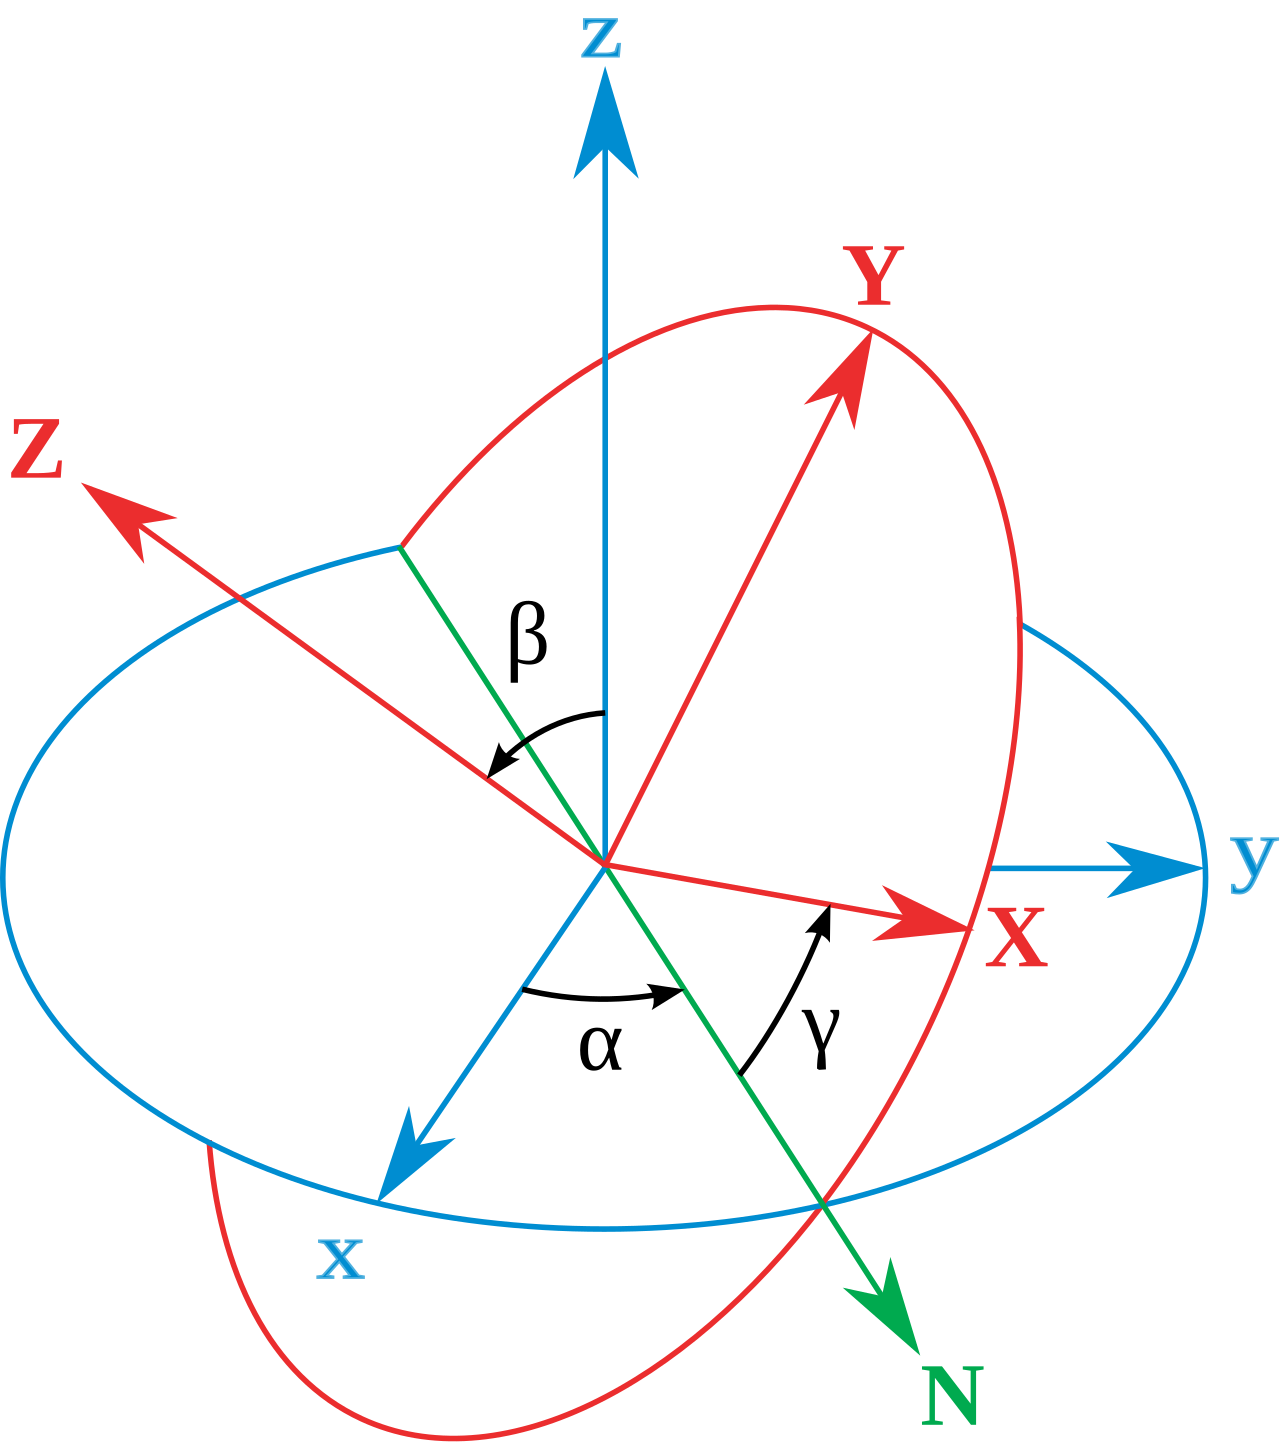
\includegraphics[width=0.65\textwidth]{Images/agent/he_toa_do_drone.png}
    \caption[Hệ tọa độ vật thể Body Frame của Quadcopter]{\bfseries\fontsize{12pt}{0pt}\selectfont Hệ tọa độ vật thể Body Frame của Quadcopter}
    \label{fig:he_toa_do_drone}
\end{figure}

Nguyên lý cân bằng và di chuyển của Quadcopter cấu hình Quad-X dựa trên chiều quay đối xứng của 4 motor (Hình \ref{fig:chieu_quay_motor}):
\begin{itemize}
    \item \textbf{Động cơ quay nghịch CCW}: Động cơ M1 (trước - phải) và M3 (sau - trái).
    \item \textbf{Động cơ quay thuận CW}: Động cơ M2 (sau - phải) và M4 (trước - trái).
\end{itemize}

\begin{figure}[H]
    \centering
    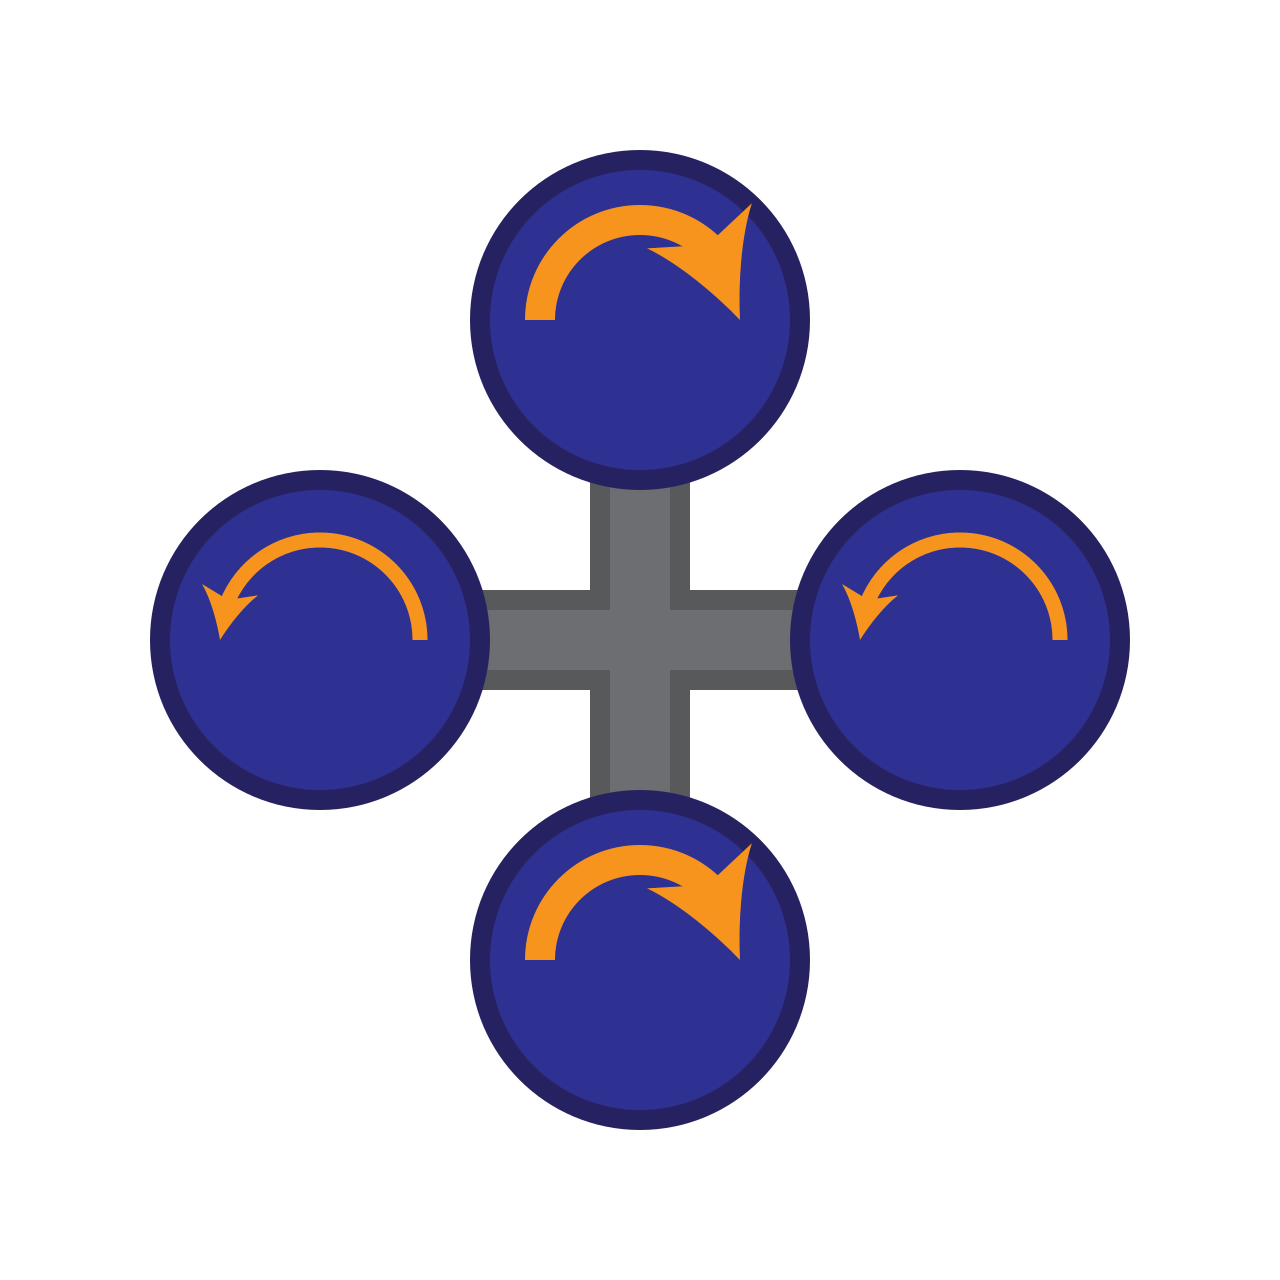
\includegraphics[width=0.65\textwidth]{Images/agent/chieu_quay_motor.png}
    \caption[Sơ đồ chiều quay động cơ cấu hình Quad-X]{\bfseries\fontsize{12pt}{0pt}\selectfont Sơ đồ chiều quay động cơ cấu hình Quad-X}
    \label{fig:chieu_quay_motor}
\end{figure}

Việc thay đổi tốc độ tương đối giữa các cặp động cơ tạo ra momen lực lệch thăng bằng để thực hiện các hành vi cơ động:
\begin{itemize}
    \item \textbf{Nghiêng phải (Roll dương)}: Tăng tốc các động cơ bên trái (M3, M4) và giảm tốc các động cơ bên phải (M1, M2).
    \item \textbf{Chúi mũi trước (Pitch âm)}: Tăng tốc các động cơ phía sau (M2, M3) và giảm tốc các động cơ phía trước (M1, M4).
    \item \textbf{Xoay trái CCW (Yaw dương)}: Tăng tốc các động cơ quay thuận CW (M2, M4) và giảm tốc các động cơ quay nghịch CCW (M1, M3). Mô-men phản lực lệch hướng sẽ làm thân drone xoay theo chiều ngược lại.
\end{itemize}

\subsection{Hệ thống điều khiển phản hồi PID vòng kín rời rạc}

Để duy trì sự cân bằng của Quadcopter trước các luồng gió nhiễu động từ môi trường bên ngoài, hệ thống nhúng liên tục chạy thuật toán điều khiển phản hồi PID vòng kín (Proportional-Integral-Derivative) trong miền rời rạc. Sơ đồ khối của bộ điều khiển được thể hiện trong Hình \ref{fig:so_do_khoi_pid}.

\begin{figure}[H]
    \centering
    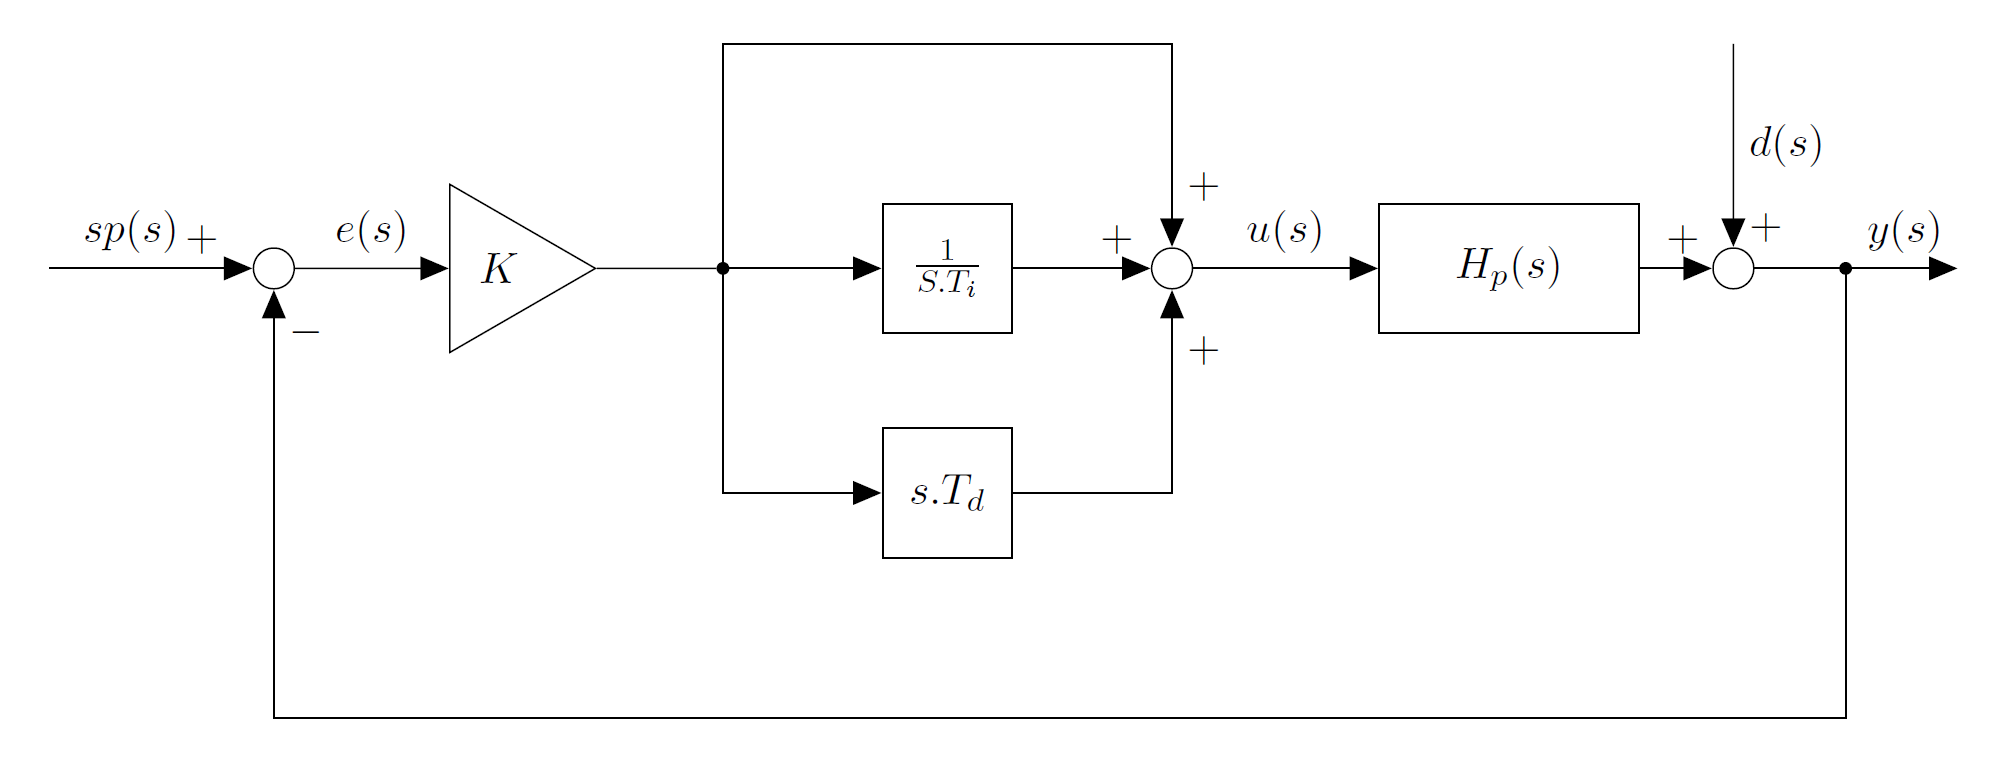
\includegraphics[width=0.85\textwidth]{Images/agent/so_do_khoi_pid.png}
    \caption[Sơ đồ khối bộ điều khiển phản hồi PID rời rạc]{\bfseries\fontsize{12pt}{0pt}\selectfont Sơ đồ khối bộ điều khiển phản hồi PID rời rạc}
    \label{fig:so_do_khoi_pid}
\end{figure}

Sai số góc nghiêng $e(t)$ tại thời điểm trích mẫu $n$ được định nghĩa bằng hiệu số giữa giá trị đặt từ tay điều khiển $Setpoint$ và góc nghiêng thực tế đo từ cảm biến $Feedback$:
\begin{equation}
    e[n] = Setpoint[n] - Feedback[n]
\end{equation}

Tín hiệu điều khiển đầu ra của khâu PID rời rạc được tính bằng công thức:
\begin{equation}
    u[n] = K_p \cdot e[n] + K_i \sum_{j=0}^{n} e[j] \cdot T + K_d \frac{e[n] - e[n-1]}{T}
\end{equation}
Trong đó, $T$ là chu kỳ trích mẫu của vòng điều khiển. Đối với hệ thống điều khiển nhúng Drone, hai hiện tượng kỹ thuật quan trọng cần được giải quyết triệt để trong firmware:

\begin{enumerate}
    \item \textbf{Hiện tượng bão hòa tích phân (Integral Windup)}: Xảy ra khi sai số lớn kéo dài khiến thành phần tích phân $I$ tăng quá mức giới hạn phần cứng của động cơ (vượt ngưỡng ga 2000$\mu s$). Khi Drone muốn đổi hướng gấp, khâu $I$ tích lũy quá lớn sẽ gây hiện tượng trễ đáp ứng nghiêm trọng, dẫn đến dao động quá đà hoặc lộn nhào (lật Drone). Thuật toán giải quyết bằng cơ chế **Anti-windup clamping** (khóa cứng giới hạn đầu ra khâu I ở mức $\pm 400$):
    \begin{equation}
        i\_mem = \max(\min(i\_mem + K_i \cdot e[n], PID\_MAX), -PID\_MAX)
    \end{equation}
    \item \textbf{Nhiễu khâu vi phân (Derivative Noise)}: Khâu vi phân cực kỳ nhạy cảm với các rung động cơ khí tần số cao của cánh quạt truyền qua khung sườn tới cảm biến IMU. Việc vi phân trực tiếp dữ liệu thô sẽ khuếch đại nhiễu làm nóng động cơ và gây cháy ESC. Hệ thống khắc phục bằng cách thiết lập **Bộ lọc thông thấp số IIR (Infinite Impulse Response)** bậc 1:
    \begin{equation}
        gyro\_input[n] = gyro\_input[n-1] \cdot 0.7 + new\_reading \cdot 0.3
    \end{equation}
\end{enumerate}

\subsection{Hệ thống cảm biến định vị quán tính IMU MPU6050 và Bộ lọc bù}

Cảm biến IMU MPU6050 \cite{mpu6050} tích hợp bộ cảm biến gia tốc 3 trục (Accelerometer) và cảm biến vận tốc góc 3 trục (Gyroscope) như mô tả trong Hình \ref{fig:truc_mpu6050}.

\begin{figure}[H]
    \centering
    
\includegraphics[width=0.45\textwidth]{Images/agent/truc_mpu6050.png}
    \caption[Sơ đồ các trục cảm biến trên chip MPU6050]{\bfseries\fontsize{12pt}{0pt}\selectfont Sơ đồ các trục cảm biến trên chip MPU6050}
    \label{fig:truc_mpu6050}
\end{figure}

Nguyên lý tính toán góc nghiêng từ cảm biến IMU có các đặc điểm đối nghịch:
\begin{itemize}
    \item \textbf{Gyroscope}: Tính góc bằng cách tích phân vận tốc góc theo thời gian: $\theta_{gyro} = \theta + \omega \cdot dt$. Khâu này phản hồi rất nhanh trước các chuyển động động học đột ngột, nhưng tích lũy sai số theo thời gian tạo ra hiện tượng trôi góc (Drift) do nhiễu offset DC của cảm biến.
    \item \textbf{Accelerometer}: Tính góc bằng công thức lượng giác dựa trên véc-tơ gia tốc trọng trường $g$:
    \begin{equation}
        \theta_{accel} = \arctan2(a_y, a_z) \cdot \frac{180}{\pi}
    \end{equation}
    Gia tốc trọng trường là mốc quy chiếu tuyệt đối nên góc tính từ accelerometer không bị trôi theo thời gian, nhưng nó cực kỳ nhạy cảm với các lực gia tốc động học của Drone lúc di chuyển và rung động cơ khí, gây nhiễu tức thời lớn.
\end{itemize}

Để dung hợp ưu điểm của hai cảm biến, hệ thống triển khai bộ lọc bù rời rạc (Complementary Filter) \cite{mahony2008} như sơ đồ trong Hình \ref{fig:bo_loc_bu}.

\begin{figure}[H]
    \centering
    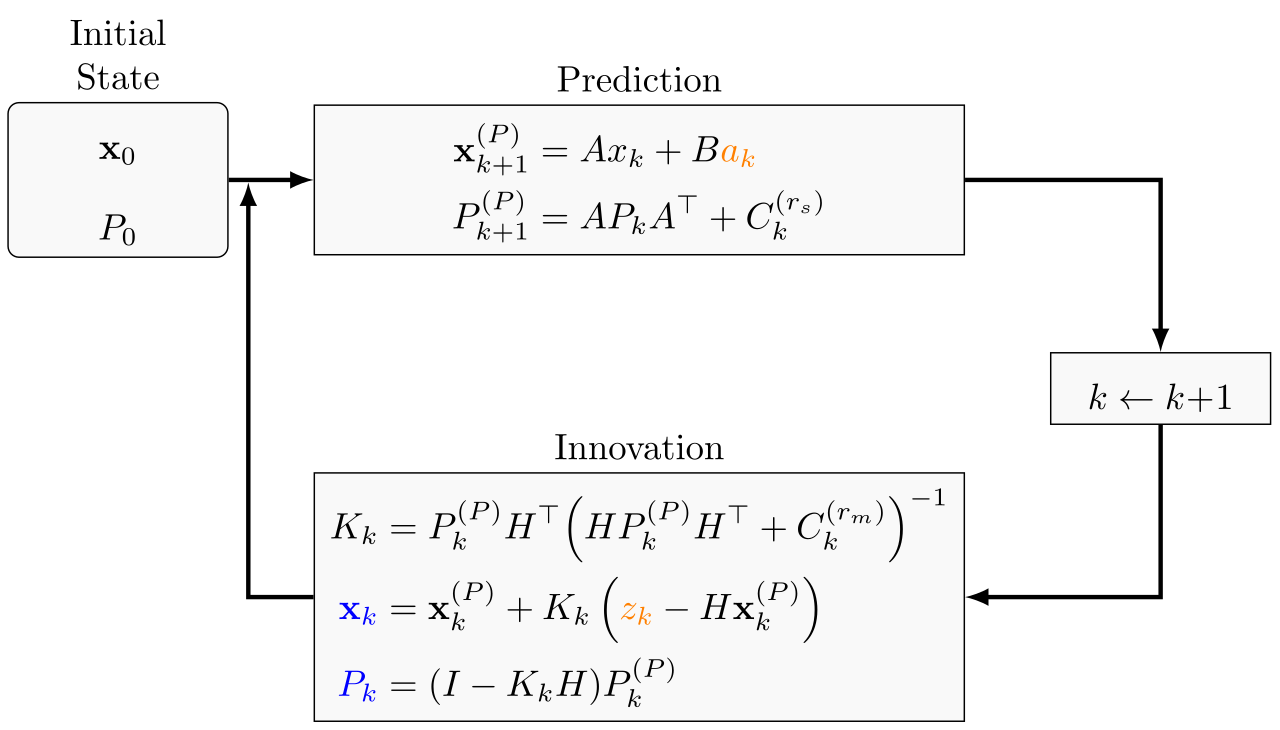
\includegraphics[width=0.8\textwidth]{Images/agent/bo_loc_bu.png}
    \caption[Sơ đồ thuật toán bộ lọc bù Complementary Filter]{\bfseries\fontsize{12pt}{0pt}\selectfont Sơ đồ thuật toán bộ lọc bù Complementary Filter}
    \label{fig:bo_loc_bu}
\end{figure}

Góc tư thế ước lượng tại mỗi chu kỳ trích mẫu được tính bằng công thức:
\begin{equation}
    \theta_{filter}[n] = \alpha \cdot (\theta_{filter}[n-1] + \omega_{gyro} \cdot dt) + (1 - \alpha) \cdot \theta_{accel}[n]
\end{equation}
Hệ số $\alpha$ được thiết lập bằng 0.98. Tỷ trọng này giúp hệ thống tin cậy 98\% vào sự thay đổi nhanh của Gyroscope trong thời gian ngắn, đồng thời liên tục lấy 2\% mốc tham chiếu tuyệt đối của Accelerometer để kéo góc lọc bù về giá trị thực, triệt tiêu hoàn toàn hiện tượng trôi góc.

\subsection{Giao thức truyền thông điều khiển vô tuyến CRSF và I2C}

ExpressLRS (ELRS) \cite{expresslrs2023} là công nghệ truyền sóng vô tuyến tầm xa mã nguồn mở hàng đầu hiện nay dựa trên công nghệ điều chế LoRa (Long Range), đem lại độ nhạy thu cực cao và khả năng xuyên nhiễu tuyệt đối. Bộ thu ELRS giao tiếp với Flight Controller thông qua giao thức truyền tin nối tiếp CRSF (Crossfire Protocol) với tốc độ baud rate tiêu chuẩn là 420.000\,bps.

Cấu trúc một khung dữ liệu CRSF được mô tả trực quan trong Hình \ref{fig:crsf_protocol}.

\begin{figure}[H]
    \centering
    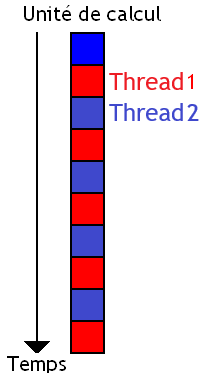
\includegraphics[width=0.85\textwidth]{Images/agent/crsf_protocol.png}
    \caption[Cấu trúc byte của khung dữ liệu giao thức CRSF]{\bfseries\fontsize{12pt}{0pt}\selectfont Cấu trúc byte của khung dữ liệu giao thức CRSF}
    \label{fig:crsf_protocol}
\end{figure}

Khung tin CRSF gồm các byte chức năng:
\begin{itemize}
    \item \textbf{Device Address (1 byte)}: Xác định đích đến (0xC8 cho Transmitter, 0xEE cho Flight Controller).
    \item \textbf{Frame Length (1 byte)}: Số lượng byte dữ liệu tiếp theo bao gồm cả byte CRC.
    \item \textbf{Type (1 byte)}: Định nghĩa loại dữ liệu (ví dụ 0x16 cho gói tin 16 kênh RC).
    \item \textbf{Payload (22 bytes)}: Chứa thông tin 16 kênh RC. Để tối ưu hóa băng thông, các kênh RC được đóng gói dưới dạng 11-bit trên mỗi kênh thay vì gửi 16-bit truyền thống.
    \item \textbf{CRC (1 byte)}: Mã kiểm tra lỗi CRC8 giúp loại bỏ hoàn toàn các khung tin bị sai lệch bit do nhiễu sóng.
\end{itemize}

Bên cạnh đó, việc lưu trữ các tham số cấu hình PID, căn chỉnh cảm biến được thực hiện qua bộ nhớ ROM EEPROM 24LC256 giao tiếp chuẩn I2C. Giản đồ xung timing của giao thức I2C được thể hiện trong Hình \ref{fig:i2c_timing}.

\begin{figure}[H]
    \centering
    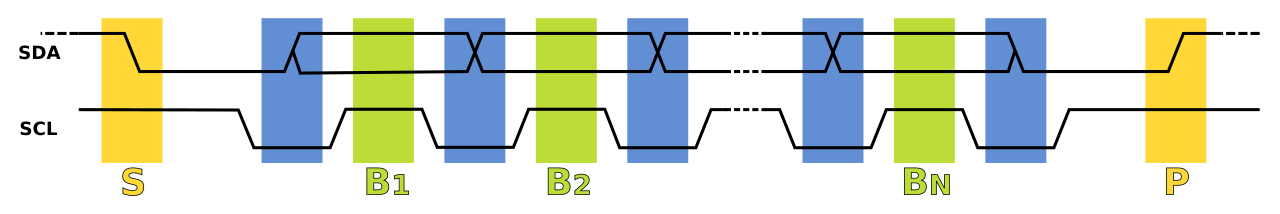
\includegraphics[width=0.85\textwidth]{Images/agent/i2c_timing.png}
    \caption[Giản đồ xung timing giao tiếp I2C giữa MCU và ngoại vi]{\bfseries\fontsize{12pt}{0pt}\selectfont Giản đồ xung timing giao tiếp I2C giữa MCU và ngoại vi}
    \label{fig:i2c_timing}
\end{figure}

Giao tiếp I2C sử dụng hai đường tín hiệu SCL (Serial Clock) và SDA (Serial Data). Cơ chế bao gồm xung START (SDA chuyển mức cao xuống thấp khi SCL cao), chuỗi bit dữ liệu đồng bộ theo nhịp clock SCL, bit ACK kiểm tra từ slave và xung STOP (SDA chuyển thấp lên cao khi SCL cao), giúp MCU ghi nhận cấu hình một cách chính xác tuyệt đối.


\subsection*{Kết luận Chương 1}
\addcontentsline{toc}{subsection}{Kết luận Chương 1}

Chương 1 đã cung cấp nền tảng lý luận toàn diện cho đề tài trên hai phương diện. Về tổng quan, chương khảo sát các nghiên cứu tiêu biểu về UAV cứu hộ trong và ngoài nước, giới thiệu chi tiết các công nghệ nền tảng được lựa chọn (STM32F103C8T6, MPU6050, ExpressLRS, VTX/VRX, YOLOv8) và xác định được ba khoảng trống nghiên cứu quan trọng cần lấp đầy. Về cơ sở lý thuyết, mô hình động lực học Newton-Euler mô tả đầy đủ chuyển động 6 bậc tự do của Quadcopter, thuật toán bộ lọc bù Complementary Filter đạt sai số ước lượng góc dưới 1\degree{}, bộ điều khiển PID kép (vòng góc -- vòng tốc độ góc) đảm bảo ổn định bay và giao thức CRSF/ELRS cung cấp kết nối điều khiển độ trễ thấp. Tất cả kết quả lý thuyết này được ứng dụng trực tiếp vào thiết kế phần cứng và lập trình firmware tại Chương 2.
